\section{Introduction}
\label{sec:intro}
%\KZ{Be careful not to use ``context'' for ``premise''. We stick to the
%terminology ``premise'' and ``choices'' throughout this paper.}
%\KZ{MCNLR is kind of tasks that is made up of
%a context and two or more choices, all in text form.
%Recently, research has noted that some advanced NLP models
%may not be truly solving this type of questions by understanding
%the underlying logical connections between the context and the choices,
%but instead resorting to local signals in the choices alone.
%Such speculations were largely fueled by a kind of
%experiments called ``end-only tests''. Although such tests
%can show that models have some ability to predict correct choices
%without given the context, it doesn't show what the model does
%if it were given the full questions with the context.
%In this work ...  }
%main point:
%1. identify short circuit, dataset have some hints, spurious feature. 
%1. pretrained models perform very well on many tasks but fail on ``stress tests'' especially 
%the cases requiring to know specific relations between context and candidates, like coreference. 
%Thus there is an assumption that model learns a lot only from candidates.
%2. previous work try to explain this by candidate-only test, but it can't really judge if the model really 
%learn from candidates.We design another test called cross test...
%3. In this paper, we further study how to improve models by some simple data augmentation methods 
%based on the weakness of models. We target to teach models to look at both context and candidates. 

%Multiple-choice questions (MCQs) are a widely used format  
%in natural language understanding tasks. 

%Large-scale neural networks have been applied extensively
%to natural language reasoning (NLR) tasks such as
%causal reasoning~\cite{roemmele2011choice}, 
%story ending prediction~\cite{roc2017},
%argument reasoning comprehension~\cite{arct2018}, and 
%reading comprehension~\cite{yu2020reclor}.
%Many of the current benchmarks of these NLR tasks take the 
%form of multiple-choice questions (MCQs) which are made up 
%of a premise and two or more choices. Below is an example taken 
%from COPA~\cite{roemmele2011choice}, which tests commonsense causal 
%reasoning.
Large-scale neural networks have been extensively 
applied to natural language reasoning (NLR) tasks, including causal reasoning~\cite{roemmele2011choice}, 
story ending prediction~\cite{roc2017}, argument reasoning comprehension~\cite{arct2018}, 
and reading comprehension~\cite{yu2020reclor}.
Many current benchmarks for these NLR tasks take the form of 
multiple-choice questions (MCQs), 
consisting of a premise and two or more choices. 
For example, the COPA dataset~\cite{roemmele2011choice} tests commonsense causal reasoning.

\begin{example}\label{ex:copa}
An MCQ from COPA:\\ \\
\noindent
\textbf{Premise:} The man hurt his back.\\
\textbf{Choice 1:} He stayed in bed for several days.  \checksymbol \\
\textbf{Choice 2:} He went to see a psychiatrist. \crosssymbol 
\end{example}

%Usually, models are trained on the training data and tested with the standard 
%validation-test split paradigm.  While accuracy on held-out data is a useful
%indicator, held-out datasets are often not diverse enough
%and may contain the same biases in the training
%data~\cite{mccoy2019right}. Furthermore, as simple aggregated statistics, 
%accuracy on the test set doesn't show the robustness of the model,
%or why a question is answered correctly. 
%There has been speculation~\cite{endingonly1,zellers2018swag} that many models 
%did not really ``understand'' the semantical and logical connection between
%the premise and the choices, 
%but do well only due to spurious statistical features in the choices, 
%which means the models are actually fragile.

Typically, models are trained on the available data and tested 
using the standard validation-test split paradigm. 
Although accuracy on held-out data is a useful indicator, 
these datasets are often insufficiently diverse and may contain 
biases present in the training data~\cite{mccoy2019right}. 
Moreover, accuracy on the test set does not fully demonstrate 
a model's robustness or provide insight into why a question is answered correctly. 
Some researchers~\cite{endingonly1,zellers2018swag,izmailov2022feature} 
have speculated that 
many models may not genuinely understand the semantic and logical 
connections between the premise and the choices, 
but perform well due to spurious statistical features in the choices. 
This suggests that the models may be fragile.

Such fragility can be observed through both white-box 
and black-box tests. In a white-box test~\cite{vig-2019-multiscale}, 
the attention map between the words in the full question 
from the final encoder layer of the model can reveal the connection, 
or lack thereof, between the premise and the choices. 
\figref{fig:att-goodex}, which displays a plot for \exref{ex:copa}, 
clearly shows that BERT does not connect the first choice 
and the premise when processing the full question. 
This phenomenon, referred to as ``short circuit'' in multiple-choice NLR, 
is the focus of this paper.


\begin{figure}[th!]
\centering
\includegraphics[width=0.35\columnwidth]{figure/end_related.eps}
\caption{Attention map showing that BERT short-circuits on a COPA question.}
\label{fig:att-goodex}
\end{figure}

%Due to the limited interpretability of deep neural models, 
Furthermore, two kinds of black-box tests have been attempted.
One is called ``ending-only tests'' in some literature~\cite{endingonly1,endingonly2}, 
which we refer to as ``choice-only test'' here since 
our focus is on MCQs.
For example, BERT, when fine-tuned on the COPA data, can answer
the question in \exref{ex:copa} correctly. When we remove the premise from 
the same question and feed it to the model, it still
gets the correct answer~(Choice 1). This result from the ``choice-only'' 
test seems to suggest that the model can make correct predictions
without even looking at the premise. 
The other blackbox test is a kind of stress test~\cite{checklist2020acl}, 
which tests if the model is short-circuiting toward (or against) certain linguistic features
such as named entities, typos, and negations.
%It breaks down potential capability failures into specific behaviors. 
In this work, we apply many stress test cases of several categories, 
and observe that many models are fragile with low accuracies.
Through the above tests, we are able to confirm that three popular 
deep models, i.e., BERT, XLNet~\cite{xlnet2019nips} and 
RoBERTa~\cite{roberta2019}, when applied to multiple-choice NLR, 
all suffer from the ``short-circuit'' problem.

%reasoning in this paper. 

%Despite the previous research advocating the choice-only test,
%we argue that it has an inherent flaw as a test for
%short circuit: just because the model answers correctly without
%the premise doesn't mean the model doesn't look into the premise
%when it's given one. What we need is a test that works with questions
%that are complete with premises and choices.
%\begin{figure}[th]
%\centering
%\includegraphics[width=\columnwidth]{figure/end_unrelated.eps}
%\caption{BERT passes the choice-only test but 
%doesn't short-circuit on another COPA question (left).}
%\label{fig:att-badex}
%\end{figure}
%
%Can we achieve the same purpose using
%the choice-only test? The answer is negative. \figref{fig:att-badex}
%shows another question which is correctly answered by BERT with
%or without the context, but the attention map shows that 
%there exists some attentions between
%the word ``forgot'' in the choice and some other words in
%the context, indicating that the model is not really short-circuiting.

%we first develop an intuitive method to visualize
%the model's attention map to verify if it is shortcircuiting. 

To reduce model short circuits, one approach is to train the models 
with hard cases resembling stress tests. 
However, the constraints of constructing choices limit 
the number of cases that can be automatically generated 
and their ability to serve as general data augmentation methods. 
Moreover, most stress tests are feature-specific and difficult to generalize. 
To address this, we propose \textit{crossover} and \textit{mutation} operators 
that can easily generate abundant data and encourage models to focus on the premise. 
When applied to augment the three models on ROC~\cite{roc2017}, COPA, ARCT~\cite{arct2018}, 
and RECLOR~\cite{yu2020reclor}, we observe up to a 42\% increase in accuracy on 
stress tests and a 10\% increase in original test data, 
outperforming the strong baseline back-translation~\cite{back2019}.


This paper makes the following contributions:
%\item We design ``crossover'' test as a blackbox proxy test to 
%massively and efficiently detect short-circuiting problem.  
%\item We propose a black-box proxy test framework for detecting short circuits, and 
%particularly ``crossover'' test which is shown to be effective in this framework.
i) we propose the crossover and mutation operations
to augment training data that teaches the models to pay attention to
the premises in questions; ii) experiments demonstrate that 
augmented models perform substantially better on diverse stress tests 
while maintaining accuracy on the original tests, indicating reduced short circuits;
iii) we provide evidence confirming that our approach indeed reduces short-circuits in these models..

%\begin{figure*}[th]
%\centering
%\begin{subfigure}[b]{0.49\textwidth}
%\centering
%\includegraphics[width=\columnwidth]{figure/end_related.eps}
%\caption{Cue ``no'' in MNLI}
%\label{fig:cue_no}
%\end{subfigure}
%\hfill
%\begin{subfigure}[b]{0.49\textwidth}
%\centering
%\includegraphics[width=\columnwidth]{figure/end_unrelated.eps}
%\caption{}
%\label{fig:cue_threw}
%\end{subfigure}
%\caption{Three test examples for distribution comparison with 4 different models}
%\label{fig:cue_result}
%\end{figure*}





%questions to discuss:
%1. how to know if a model only pay attention to candidates only? ending only? cross? 
%2. how to know if a model have a poor performance on stress test?
%word swap  choice swap(premise) reflecility (aug merge)
%3. how to explain typo and synonym? should we use grammar to test? do we have other relational stress tests?
%we only have pronoun, negation, ner now. adverbial, synonym paraphrase right to right, typo
%4. experiment should try on different test cases many times or same cases many times?
